\section{Auswertung}
\label{sec:Auswertung}

% \begin{figure}
%   \centering
%   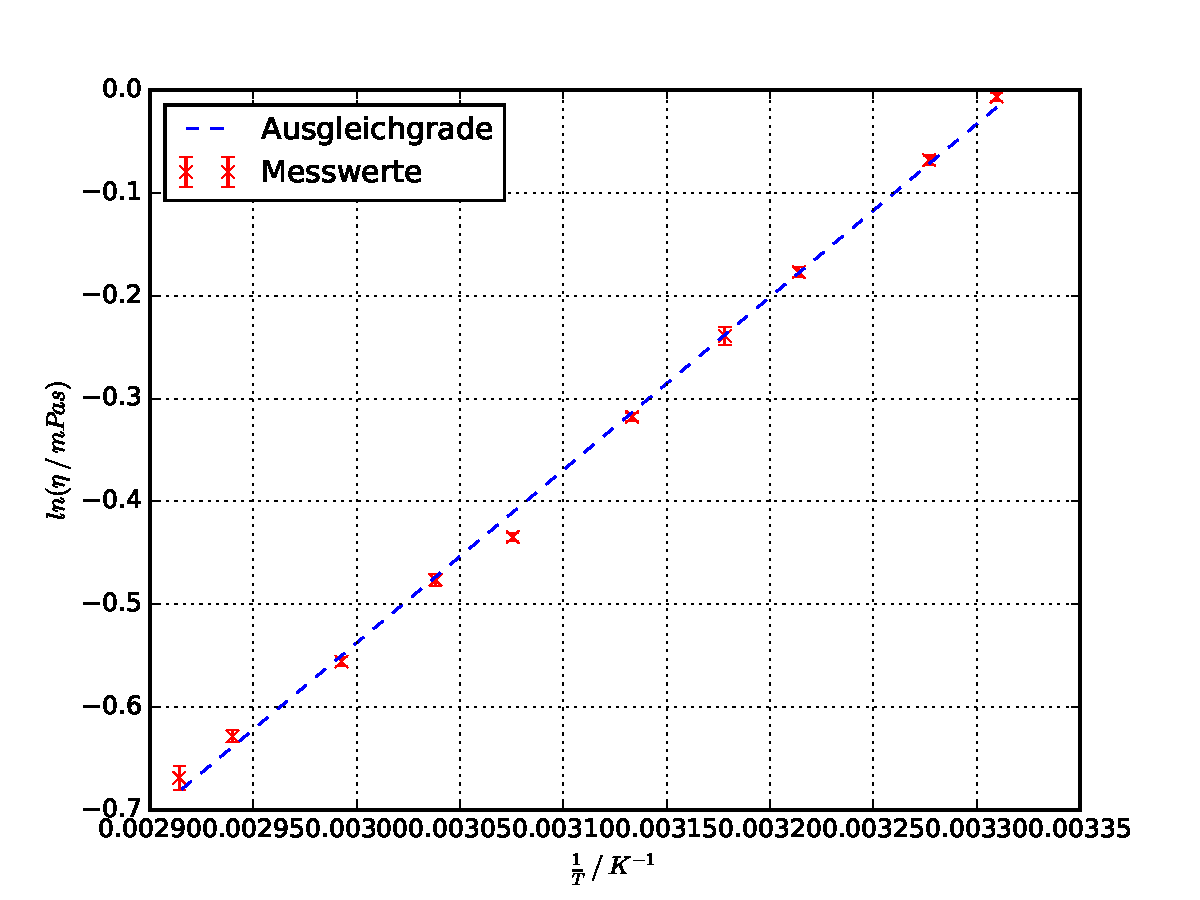
\includegraphics{plot.pdf}
%   \caption{Plot.}
%   \label{fig:plot}
% \end{figure}

\subsection{Methoden}
Alle Mittelwerte und deren Fehler wurden mit der Formel
\begin{equation}
  \langle x \rangle = \frac{1}{n} \sum_{i=1} ^{n} x_i \quad \text{und} \quad
  \Delta x = \sqrt{\frac{1}{n(n-1)} \sum_{i=1}^n (x_i - \langle x \rangle )^2}
  \label{eqn:MW}
\end{equation}
berechnet \cite{Tipler}.
\subsection{Dampfdruck und die mittlere freie Weglänge}
Die Werte für Dampfdruck und mittlerer freier Weglänge wurden mit den Formeln
\eqref{eqn:p} und \eqref{eqn:Weg} berechnet.
In der Tabelle \ref{tab:ue} sind die Temperturen, Dampfdrücke, mittlere Weglängen
sowie der Größenfaktor $ \sfrac{a}{\bar{w}}$ dargestellt, wobei $a = 1 \si{\centi \meter}$ bei
der verwendeten Versuchapparatur beträgt. Die Tabelle zeigt die Werte zweilenweise für
die verschieden Versuchsteile, d.h. die ersten beiden Zeilen zeigen die Werte für
die Messung der integralen Energieverteilung bei verschiedenen Temperturen, die Dritte
für die Messung der Franck-Hertz-Kurve und die vierte für die Messung de Ionisierungsspannung.
Der Größenfaktor sollte zischen 1000 und
4000 liegen, da sonst keine ausreichend große Stoßwahrscheinlichkeit gewährleistet ist.
Aus der Tabelle \ref{tab:ue} ist also zu entnehmen, dass nur bei der Messung
der integrale Energieverteilung eine ausreichende
Stoßwahrscheinlichkeit gewährleitstet war und bei der Messung der Franck-Hertz-Kurve
wesentlich zu hoch war.

\begin{table}
  \centering
  \caption{Temperaturen, Dampfdrücke , mittlere freie Weglängen und Größenfaktor von
  \texorpdfstring{$a$}{math} und \texorpdfstring{$\bar{w}$}{math} im Überlick }
  \sisetup{ round-mode = places, round-precision = 2 ,table-format = +3.2e+2}
  \begin{tabular}{S[scientific-notation = fixed , fixed-exponent = 0] S S S[scientific-notation = fixed , fixed-exponent = 0]}
    \toprule
    $T$ / \si{\kelvin} & $p_{sät}$ / \si{\milli \bar} & $\bar{w}$ / \si{\centi \meter} & $\frac{a}{\bar{w}} $ \\
    \midrule
    2.963499999999999659e+02 & 4.610353052222010764e-03 & 6.290190723251254390e-01 & 1.589776914559314136e+00\\
    4.321499999999999773e+02 & 6.764590844732246921e+00 & 4.287029425080899009e-04 & 2.332617532666292391e+03\\
    4.711499999999999773e+02 & 2.524846657539852046e+01 & 1.148584604668898143e-04 & 8.706367784620180828e+03\\
    3.761499999999999773e+02 & 6.331184373651318475e-01 & 4.580501575769957597e-03 & 2.183167025397006569e+02\\
    \bottomrule
  \end{tabular}
  \label{tab:ue}
\end{table}
\subsection{Differentielle Energieverteilung}
Zur Bestimmung der differentielle Energieverteilung wurde die Steigung $\frac{I_A}{U_A} $
des Graphen
der gemessenen integralen Energieverteilung gemessen und gegen die Bremsspannung $U_A$
aufgetragen. Dabei wurden die Werte erst in Centimetern bestimmt und dann wurden
die x-Achsen Skalenwerte gemittelt, für die y-Achse wurde ein Referenzwert des Maximums
genommen um einen Umrechnungsfaktor zu berechnen. Dann ergibt sich für die gemittelten
x-Achsen Skalenwerte $  (2,3 \pm 0,04)\si{\volt \per \centi \meter} $,
aus dem Referenzwert für die y-Achse ergibt sich der Wert $ 0,37 \si{\nano \ampere\per\centi \meter}$
somit ergibt sich der Umrechnungsfaktor für die Steigung mit $(1,62 \pm 0.03)\cdot 10^{-10}
\si{\ampere \per \volt} $. Auf Ablesefehler wurde verzichtet.

\begin{table}
  \centering
  \sisetup{round-mode = places, round-precision = 2}
  \resizebox{\textwidth}{!}{
  \begin{tabular}{S S[scientific-notation = fixed , fixed-exponent = 0] S@{$ \; \pm$} S S@{${}\pm{}$} S}
    \toprule
     $\frac{\Delta x}{\Delta y} $& $x$ / \si{\centi \meter} &
    \multicolumn{2}{c}{$ \frac{I_A}{U_A} \pm \frac{\Delta I_A}{\Delta U_A} $ / \si{\ampere \per \volt}  } &
    \multicolumn{2}{c}{$ U_A / \si{\volt}$} \\
    \midrule
    1.612999999999999851e-02 & 3.100000000000000089e+00 & 2.617074934306826662e-12 & 4.669846701839564058e-14 & 1.344902386117136972e+00 & 2.399812053440020243e-02\\
    2.940999999999999864e-02 & 9.599999999999999645e+00 & 4.771740472285416881e-12 & 8.514580998208405277e-14 & 4.164859002169198021e+00 & 7.431676036459416990e-02\\
    5.881999999999999729e-02 & 1.390000000000000036e+01 & 9.543480944570833761e-12 & 1.702916199641681055e-13 & 6.030368763557484968e+00 & 1.076044759445686505e-01\\
    1.304299999999999904e-01 & 1.590000000000000036e+01 & 2.116212546073400153e-11 & 3.776119685808645051e-13 & 6.898047722342734112e+00 & 1.230871343538591095e-01\\
    1.499999999999999944e-01 & 1.750000000000000000e+01 & 2.433733664885456070e-11 & 4.342696870898541232e-13 & 7.592190889370933782e+00 & 1.354732610812914573e-01\\
    2.999999999999999889e-01 & 1.850000000000000000e+01 & 4.867467329770912140e-11 & 8.685393741797082465e-13 & 8.026030368763558798e+00 & 1.432145902859366937e-01\\
    2.999999999999999889e-01 & 1.950000000000000000e+01 & 4.867467329770912140e-11 & 8.685393741797082465e-13 & 8.459869848156182925e+00 & 1.509559194905819302e-01\\
    5.500000000000000444e-01 & 2.050000000000000000e+01 & 8.923690104580005482e-11 & 1.592322185996132004e-12 & 8.893709327548808830e+00 & 1.586972486952271666e-01\\
    1.000000000000000000e+00 & 2.150000000000000000e+01 & 1.622489109923637337e-10 & 2.895131247265694222e-12 & 9.327548806941432957e+00 & 1.664385778998723753e-01\\
    3.250000000000000000e+00 & 2.250000000000000000e+01 & 5.273089607251821409e-10 & 9.409176553613505515e-12 & 9.761388286334057085e+00 & 1.741799071045176117e-01\\
    6.700000000000000178e+00 & 2.260000000000000142e+01 & 1.087067703648837137e-09 & 1.939737935668015222e-11 & 9.804772234273320564e+00 & 1.749540400249821326e-01\\
    6.700000000000000178e+00 & 2.280000000000000071e+01 & 1.087067703648837137e-09 & 1.939737935668015222e-11 & 9.891540130151845744e+00 & 1.765023058659111743e-01\\
    6.700000000000000178e+00 & 2.300000000000000000e+01 & 1.087067703648837137e-09 & 1.939737935668015222e-11 & 9.978308026030369149e+00 & 1.780505717068402161e-01\\
    2.700000000000000178e+00 & 2.350000000000000000e+01 & 4.380720596793820990e-10 & 7.816854367617375329e-12 & 1.019522776572668299e+01 & 1.819212363091628482e-01\\
    \bottomrule
  \end{tabular}
  }
\end{table}
\FloatBarrier
Die Werte die in
\begin{figure}
  \centering
  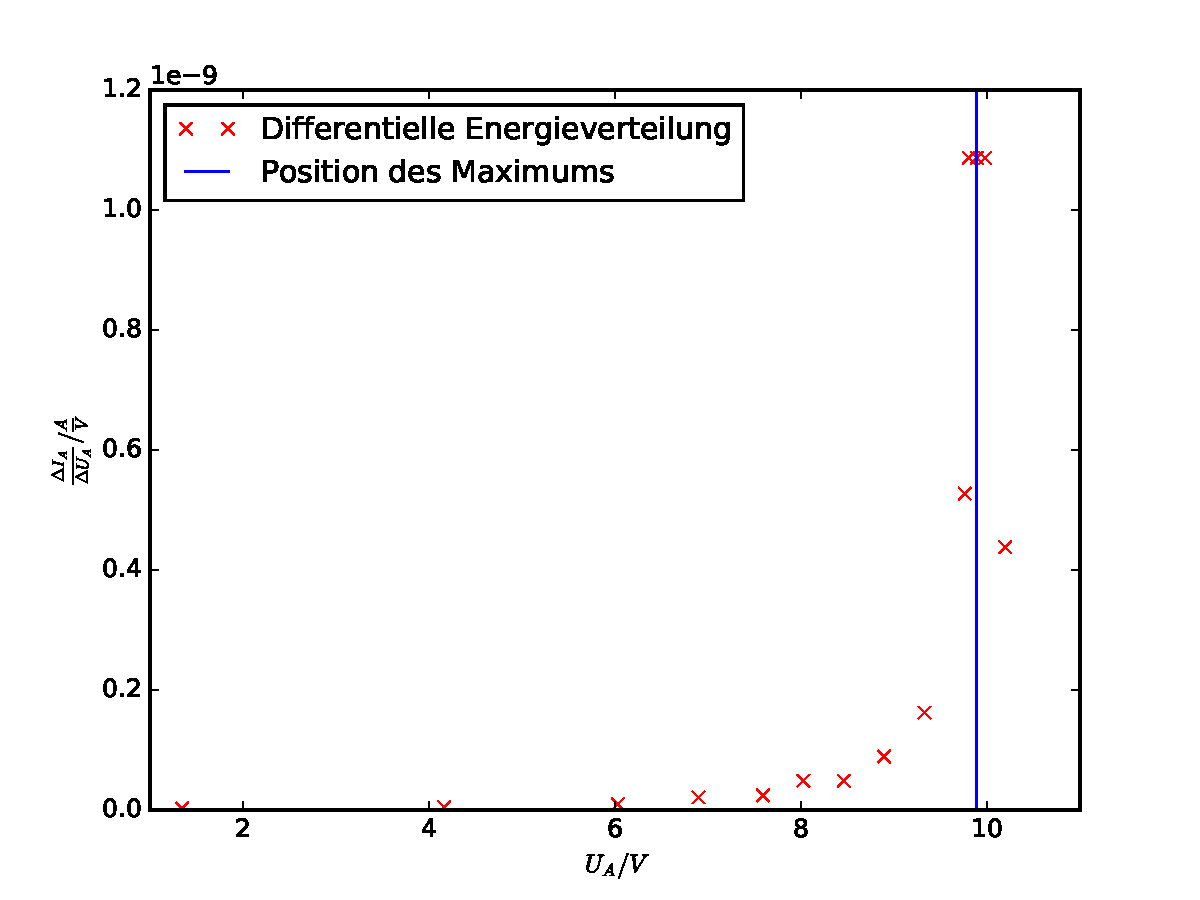
\includegraphics[height = 7cm]{plots/8a1plot.pdf}
  \caption{Differentielle Energieverteilung bei 296.35 \si{\kelvin}}
  \label{fig:8a1p}
\end{figure}

\begin{landscape}
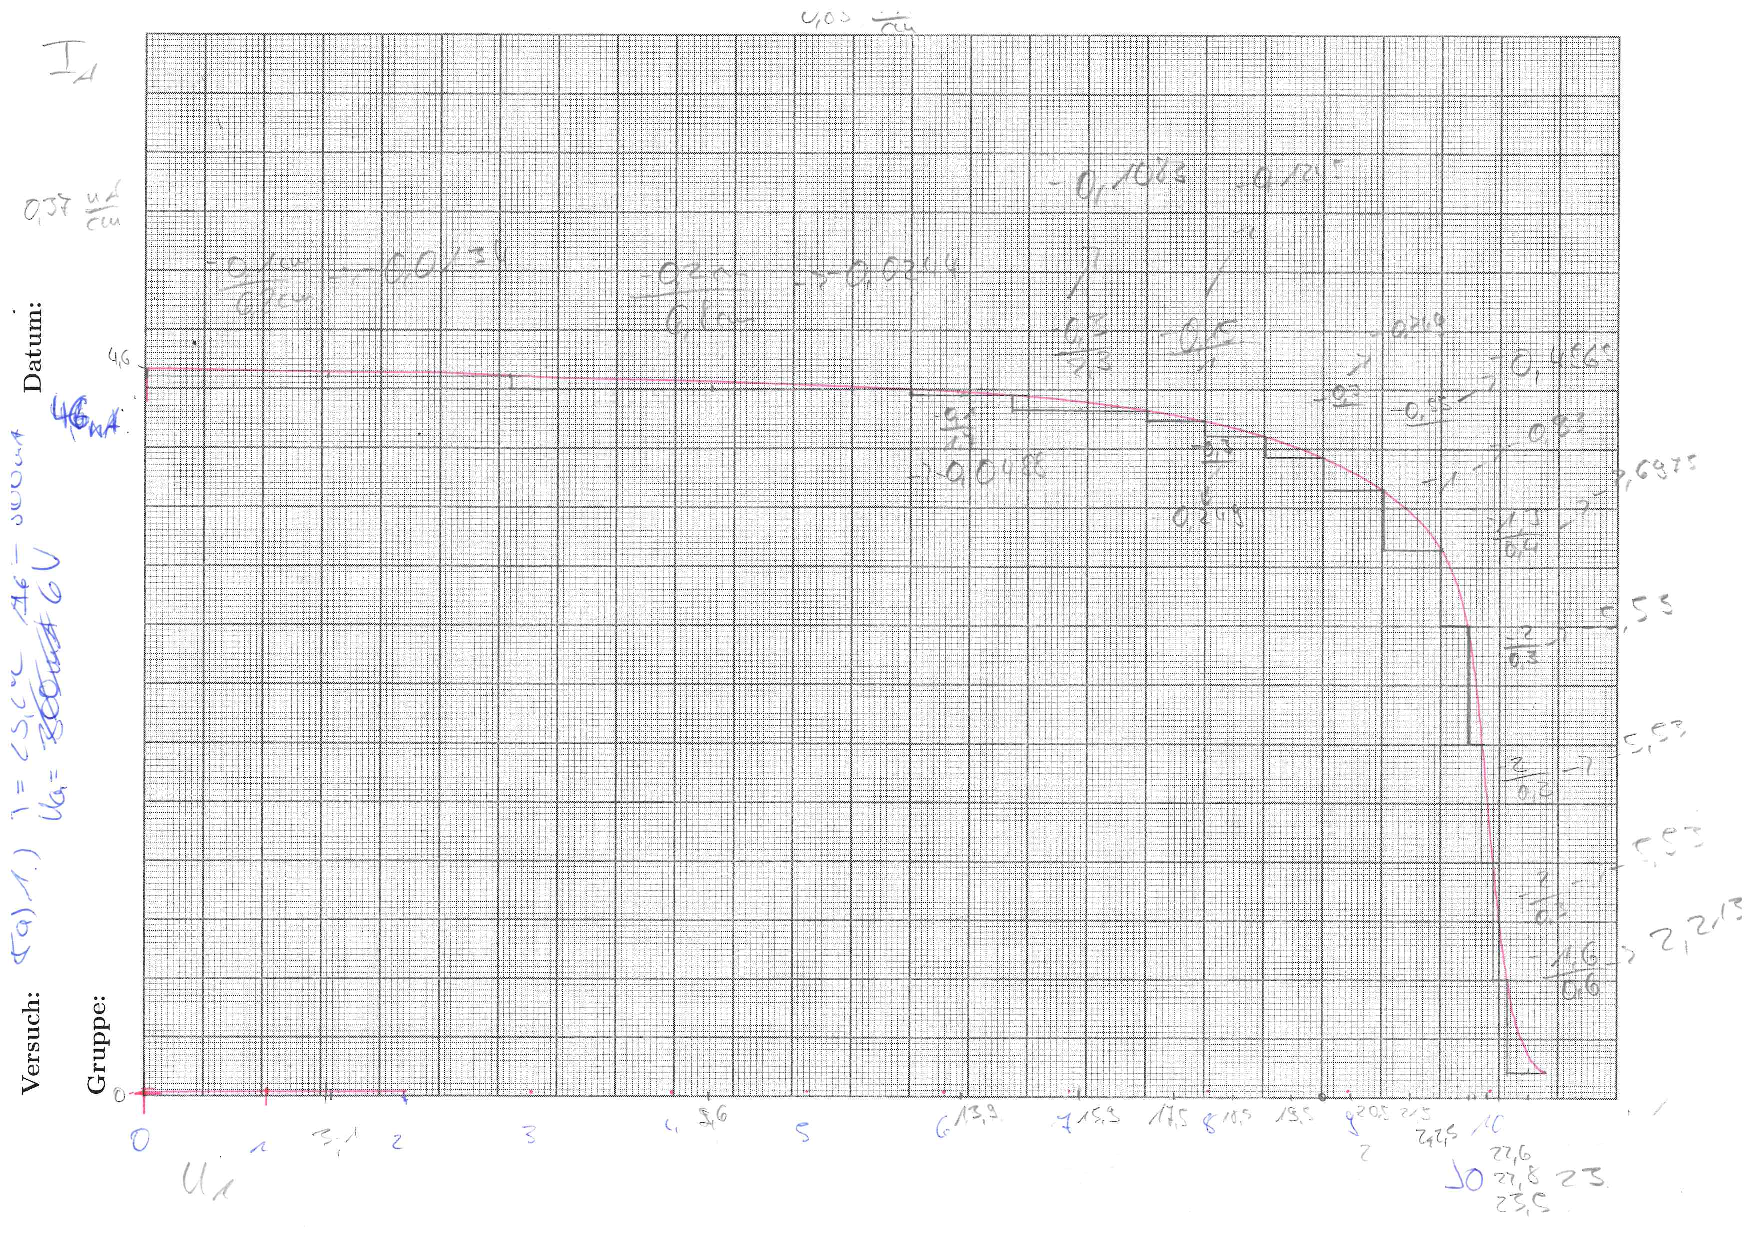
\includegraphics[page = 1, scale = 0.5]{8a1.pdf}
\label{fig:8a1}
\end{landscape}
\begin{landscape}
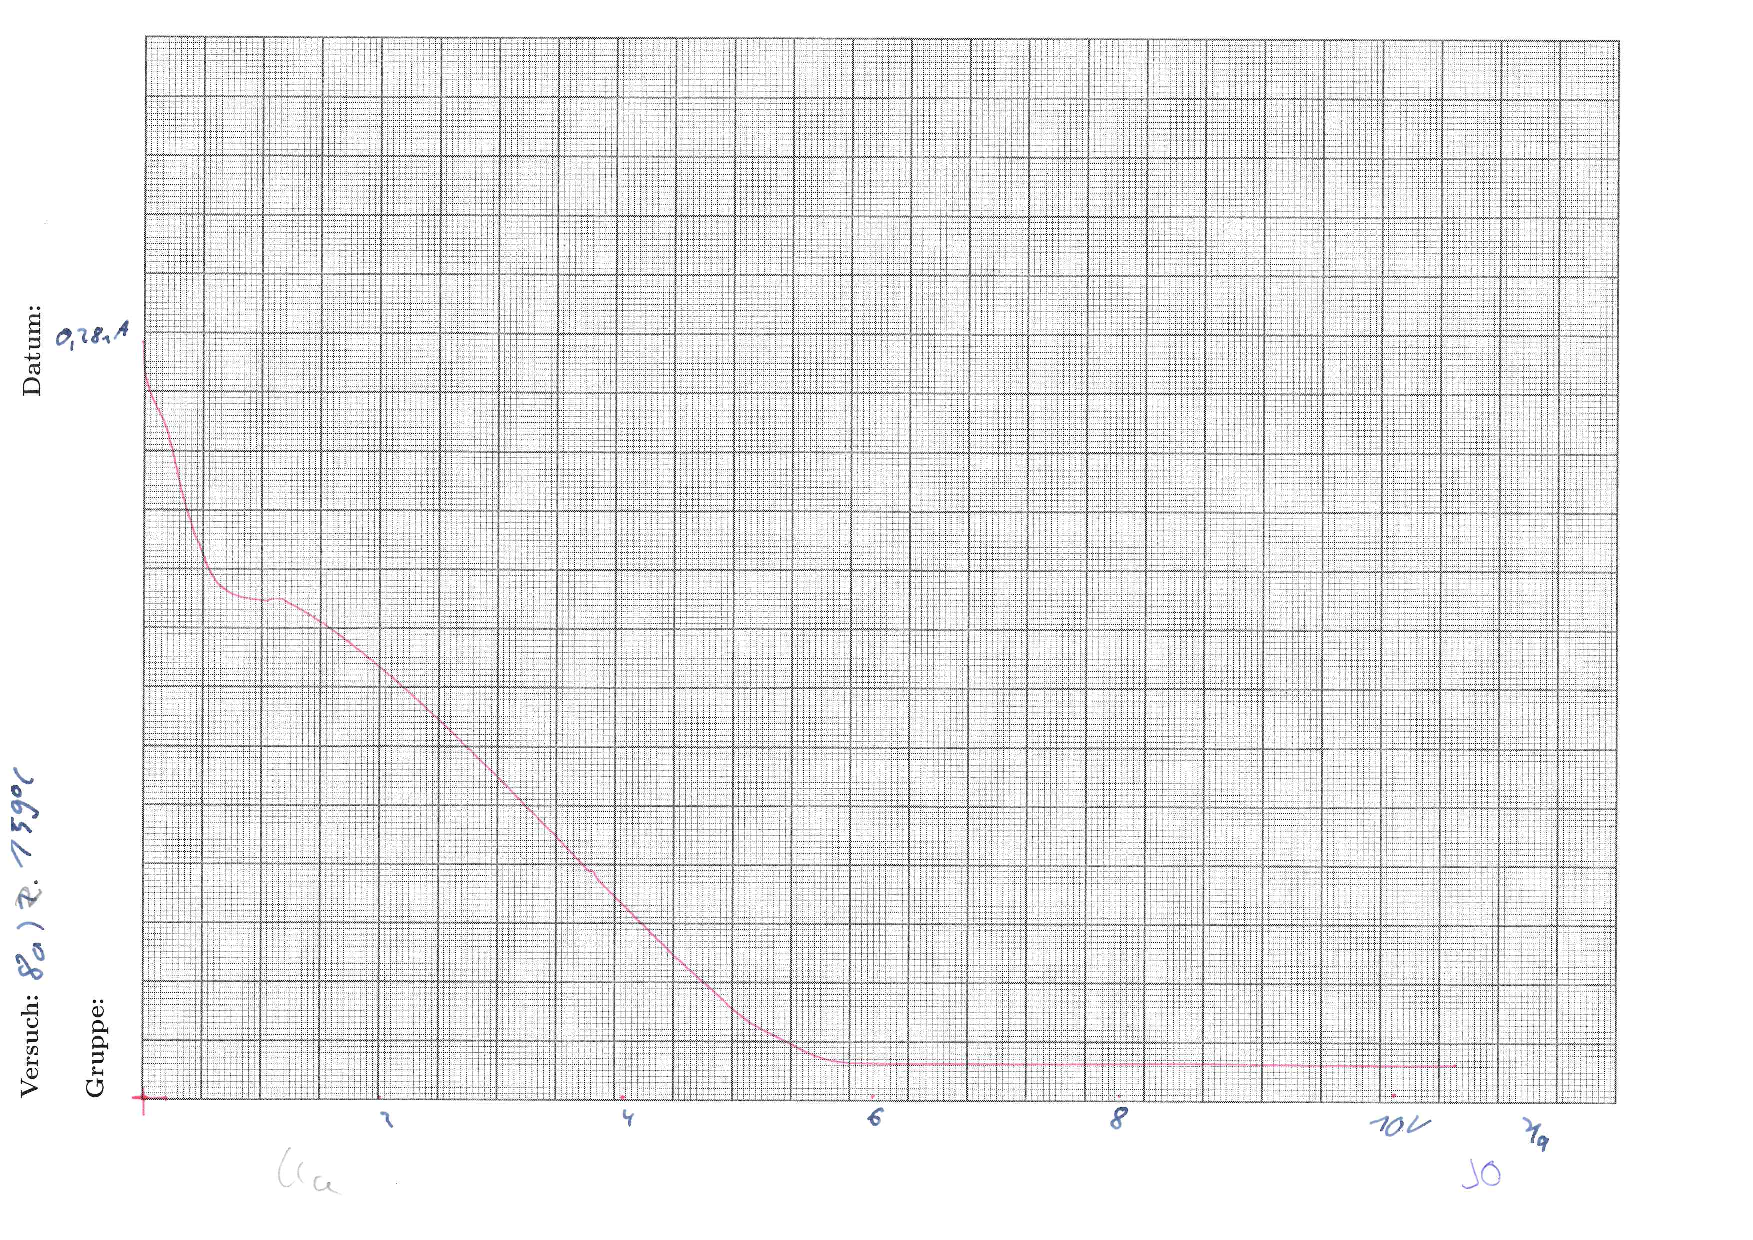
\includegraphics[page = 1, scale = 0.5]{8a2.pdf}
\label{fig:8a2}
\end{landscape}
\subsection{Franck-Hertz Kurve}
\begin{landscape}
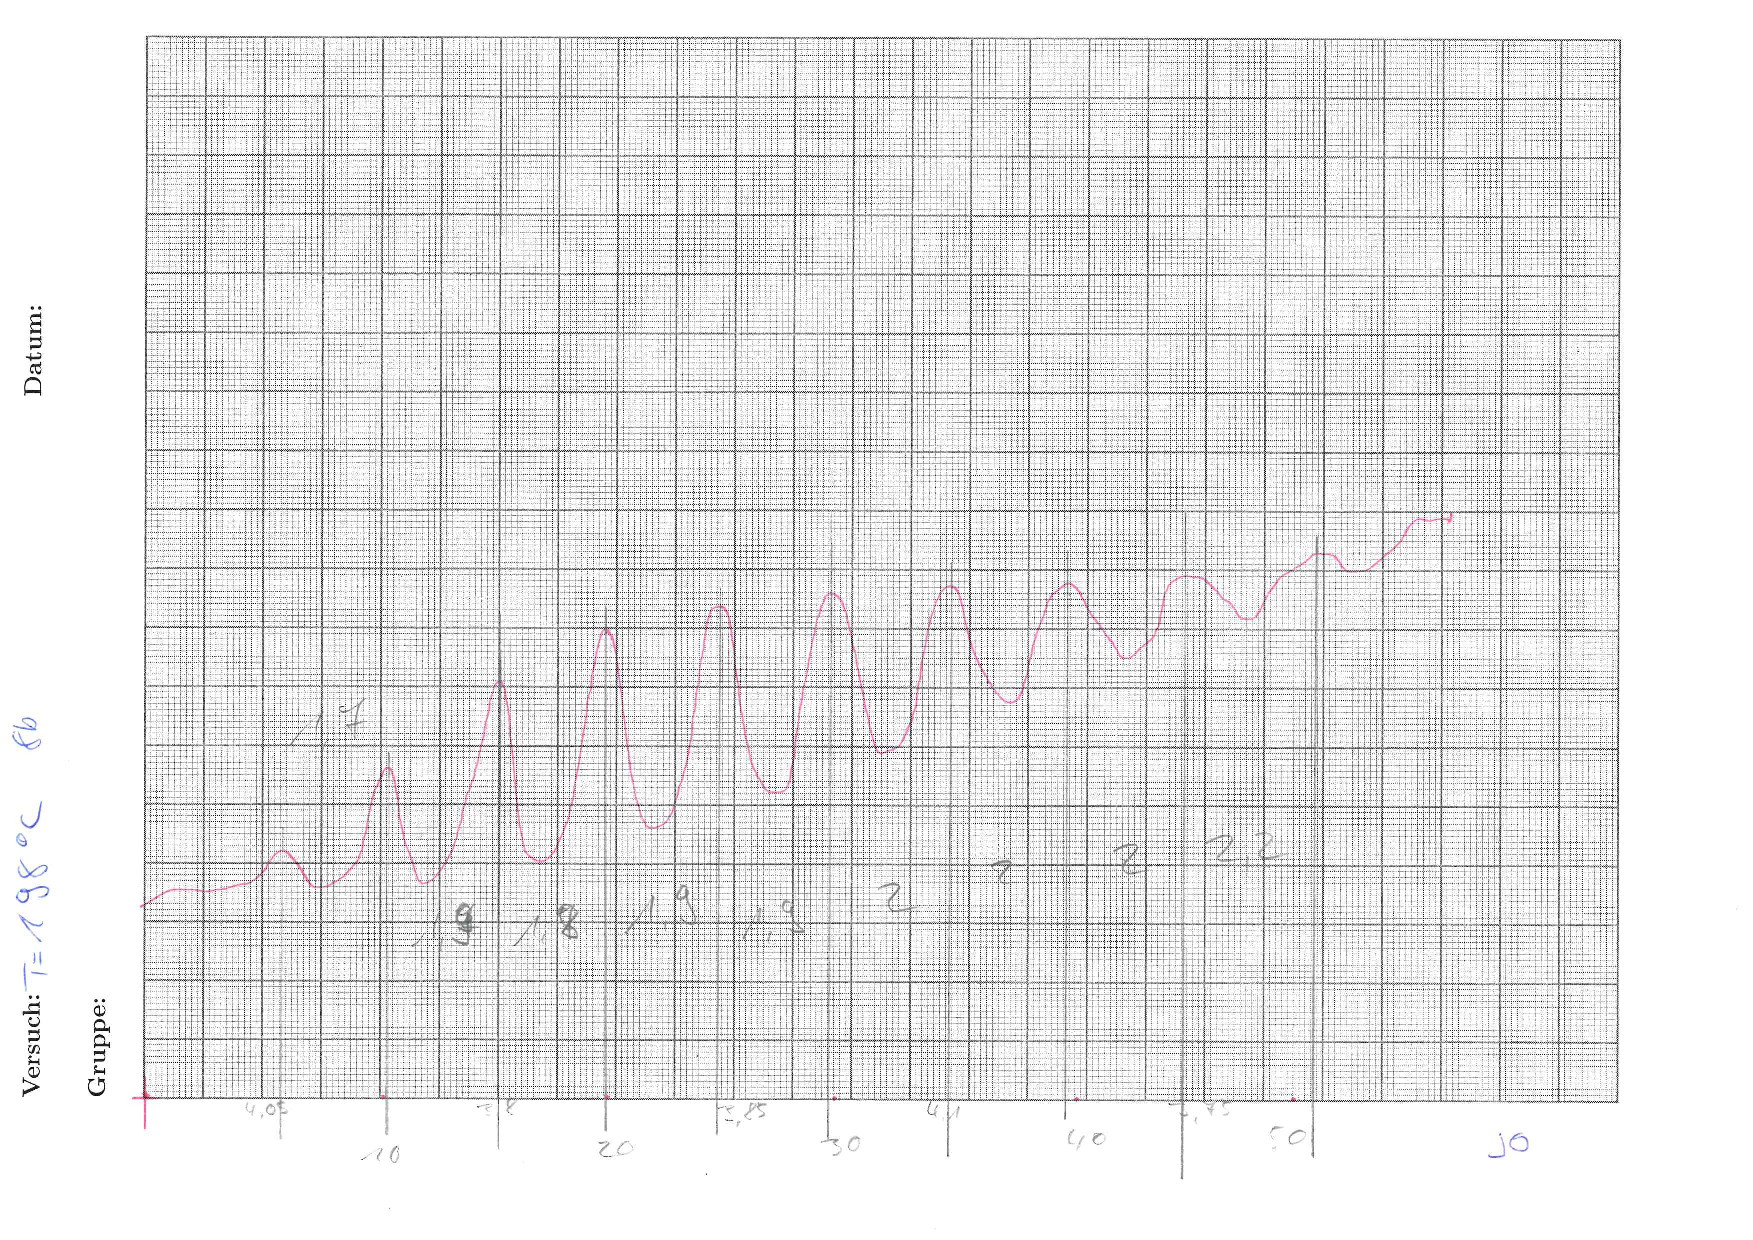
\includegraphics[page = 1, scale = 0.5]{8b.pdf}
\label{fig:8b}
\end{landscape}
\subsection{Ionisierung}
\begin{landscape}
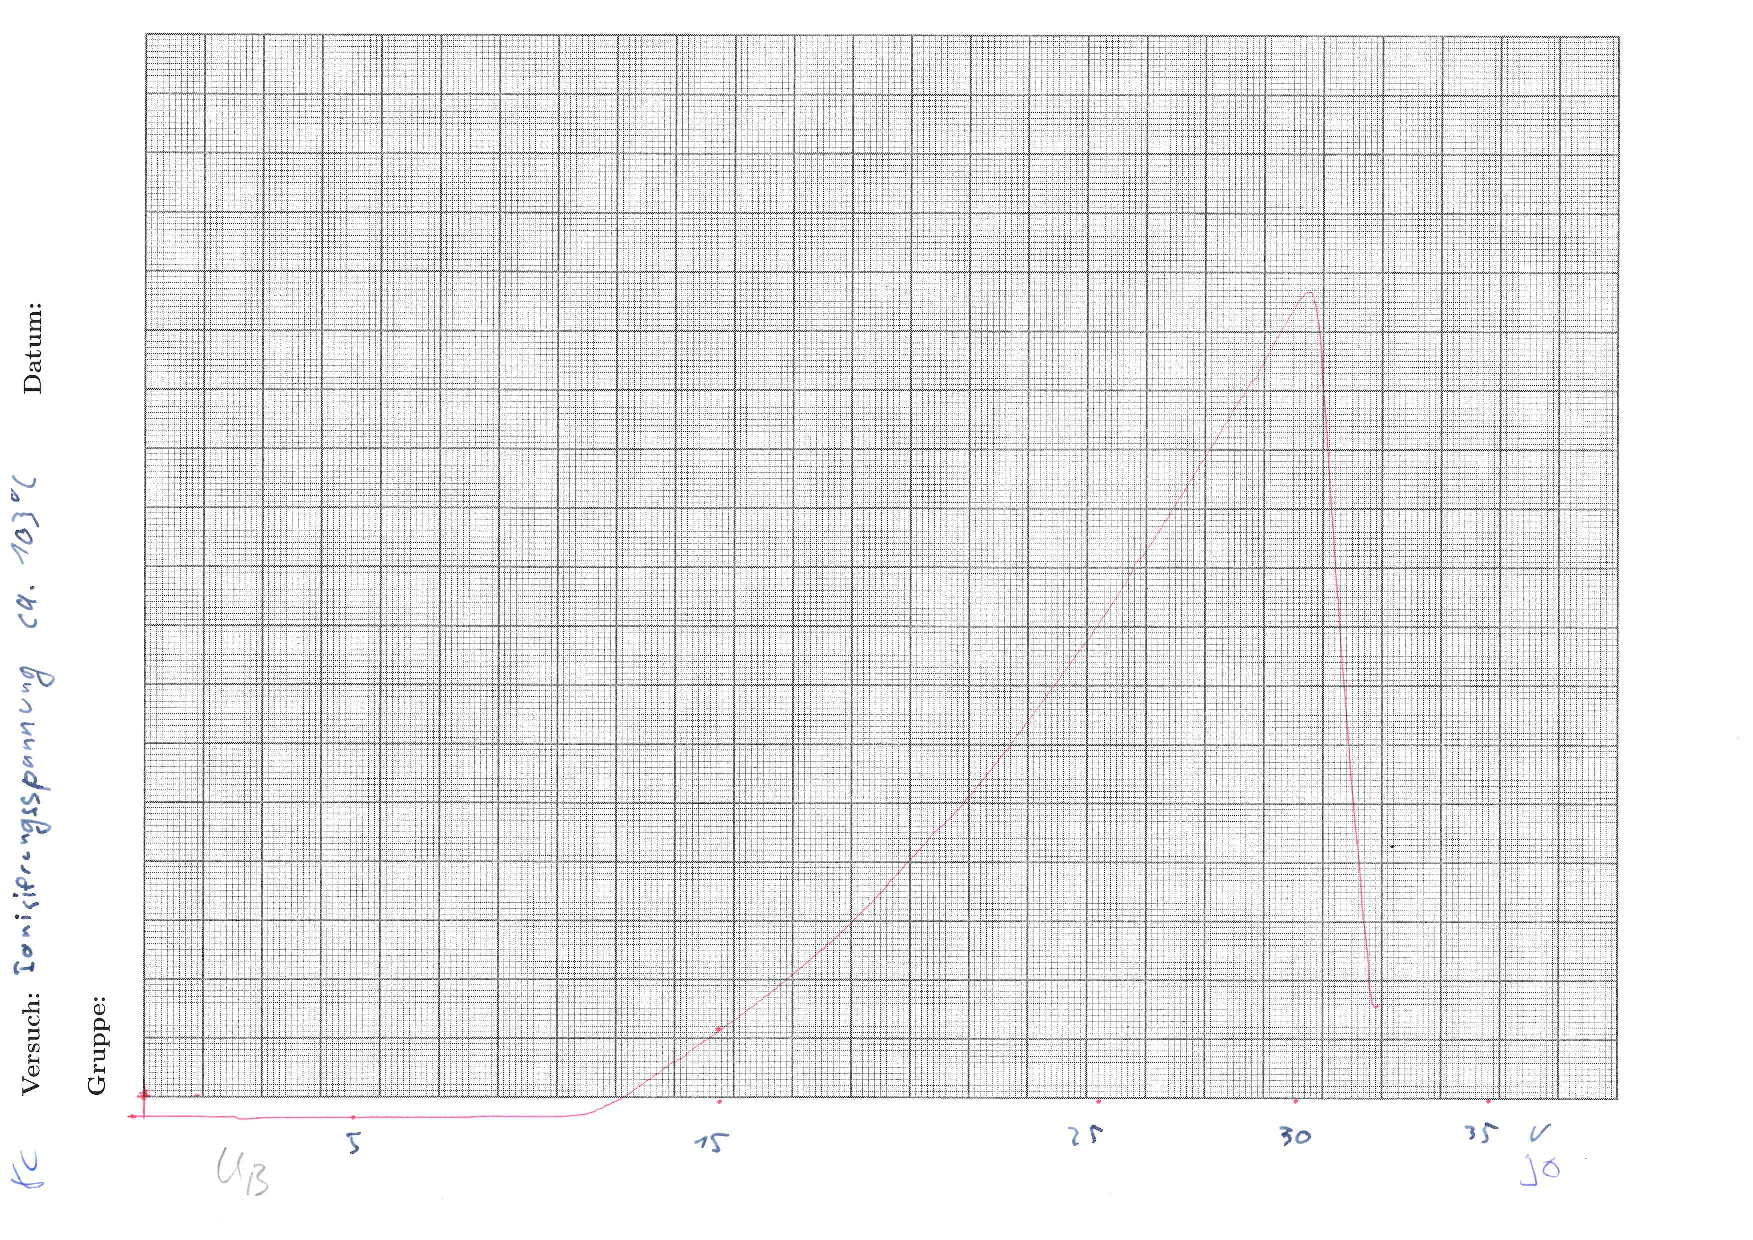
\includegraphics[page = 1, scale = 0.5]{8c.pdf}
\label{fig:8c}
\end{landscape}
